% $> xelatex emv.redes-neuronales.presentacion.tex
% o bien
% $> lualatex emv.redes-neuronales.presentacion.tex
\documentclass[spanish]{beamer}

\usepackage[es-tabla]{babel}

\usepackage{graphics,tikz}
\usetikzlibrary{automata, positioning, arrows}

\usepackage{pgfplotstable}
\pgfplotsset{compat=1.16}

\usepackage{adjustbox}
\usepackage{booktabs}
\usepackage{multirow}
\usepackage{enumitem}
\usepackage{caption}
\usepackage{subcaption}

% Matemáticas

\usepackage{amsmath, amsthm, amssymb}
\usepackage{mathtools}
\usepackage{commath}

%%% FUENTES

\usepackage[no-math]{fontspec}
\setmainfont{Libertinus Serif}
\setsansfont{Libertinus Sans}
\setmonofont{Libertinus Mono}

\usepackage[math-style=TeX]{unicode-math}
\setmathfont{Libertinus Math}

\usepackage{pifont}
\newcommand{\cmark}{\ding{51}}%
\newcommand{\xmark}{\ding{55}}%

%%% COLORES

\definecolor{background}{HTML}{F5F5F4}
\definecolor{foreground}{HTML}{3F3F3F}
\definecolor{strings}{HTML}{ED982C}
\definecolor{operators}{HTML}{CF4818}
\definecolor{identifiers}{HTML}{9A71BA}
\definecolor{keywords}{HTML}{5486C8}
%\definecolor{keywords}{HTML}{54BFC7}
\definecolor{numbers}{HTML}{80951D}
\definecolor{comments}{HTML}{AFAFAF}

%%% LISTINGS

\usepackage{listings}

\lstset{
  numbers=left,
  belowcaptionskip=1\baselineskip,
  basicstyle=\scriptsize\ttfamily\color{foreground},
  keywordstyle=\color{keywords},
  commentstyle=\color{comments},
  stringstyle=\color{strings},
  identifierstyle=\color{identifiers},
  numberstyle=\color{foreground},
  xleftmargin=2em,
  framexleftmargin=1.5em,
  breaklines=true,
  showstringspaces=false,
  tabsize=2
}

% Bibliografía

\usepackage[sorting=none, style=apa, isbn=true]{biblatex}
\DefineBibliographyStrings{spanish}{
  urlseen = {Consultado},
  retrieved = {Consultado},
}
\addbibresource{bibliografia.bib}

%%% AJUSTES DE BEAMER

%\usefonttheme{professionalfonts}

\setlength{\leftmargini}{0cm}
\setlength{\leftmarginii}{2em}

\setbeamertemplate{navigation symbols}{}

\setbeamerfont{title}{series=\bfseries}

%\setbeamertemplate{frametitle}{\color{foreground}\vspace*{1cm}\bfseries\insertframetitle\par\vskip-6pt}
\setbeamerfont{frametitle}{series=\bfseries}
\setbeamercolor{frametitle}{fg=foreground}
\setbeamerfont{framesubtitle}{size=\normalfont\small}
\setbeamercolor{framesubtitle}{fg=foreground}

\setbeamercolor{background canvas}{bg=background}

\setbeamercolor{normal text}{fg=foreground}
\setbeamercolor{alerted text}{fg=foreground}
\setbeamercolor{block title}{fg=foreground}
\setbeamercolor{alerted text}{fg=foreground}

\setbeamercolor{itemize item}{fg=foreground}
\setbeamercolor{enumerate item}{fg=foreground}

\setbeamertemplate{itemize items}[circle]
\setitemize{
  label=\usebeamerfont*{itemize item}
  \usebeamercolor[fg]{itemize item}
  \usebeamertemplate{itemize item}
}

\setbeamercolor*{title}{fg=foreground}
\setbeamercolor{qed symbol}{fg=foreground}

\usebeamercolor[fg]{normal text}

\setbeamertemplate{footline}[frame number]
\setbeamerfont{page number in head/foot}{size=\small}

\setbeamercolor{section in toc}{fg=foreground}
\setbeamerfont{section in toc}{series=\bfseries}

\setbeamercolor{caption name}{fg=foreground}
\setbeamerfont{caption name}{series=\bfseries}

\setbeamercolor{bibliography entry note}{fg=foreground}
\setbeamercolor{bibliography entry author}{fg=foreground!40!black}

\hypersetup{
  colorlinks=true,
  citecolor=numbers,
  urlcolor=operators,
  linkcolor=foreground
}

%%% INFORMACIÓN DEL DOCUMENTO

\title{Redes neuronales artificiales}
\subtitle{Estadística Multivariante}
\author{
  Johanna Capote Robayna\texorpdfstring{\\}{}
  Antonio Coín Castro\texorpdfstring{\\}{}
  Guillermo Galindo Ortuño\texorpdfstring{\\}{}
  José María Martín Luque\texorpdfstring{\\}{}
  Luis Antonio Ortega Andrés\texorpdfstring{\\}{}
  Cristina de la Torre Villaverde
}
\institute{\normalsize Universidad de Granada}
\date{20 de enero de 2020}

\begin{document}

\maketitle

\begin{frame}{Índice}
  \tableofcontents
\end{frame}

\section{Redes neuronales biológicas}

\begin{frame}{Redes neuronales biológicas}
  \begin{itemize}
    \item Ciencia cognitiva: estudio científico de la mente y sus procesos.
    \item Conexionismo: los fenómenos mentales pueden describirse mediante redes compuestas por unidades sencillas e interconectadas entre sí.
    \item Para entender cómo funciona una red neuronal artificial es útil comprender primero cómo funcionan las redes neuronales biológicas.
  \end{itemize}
\end{frame}

\begin{frame}{Redes neuronales biológicas}
  \begin{itemize}
    \item Neuronas: células básicas que componen el sistema nervioso.
    \item Dos partes diferenciadas: cuerpo celular y axón.
    \item Dendritas: receptores de señales.
    \item Axón: emisor de señales.
  \end{itemize}
\end{frame}

\begin{frame}{Redes neuronales biológicas}
  \begin{figure}[b]
    \centering
    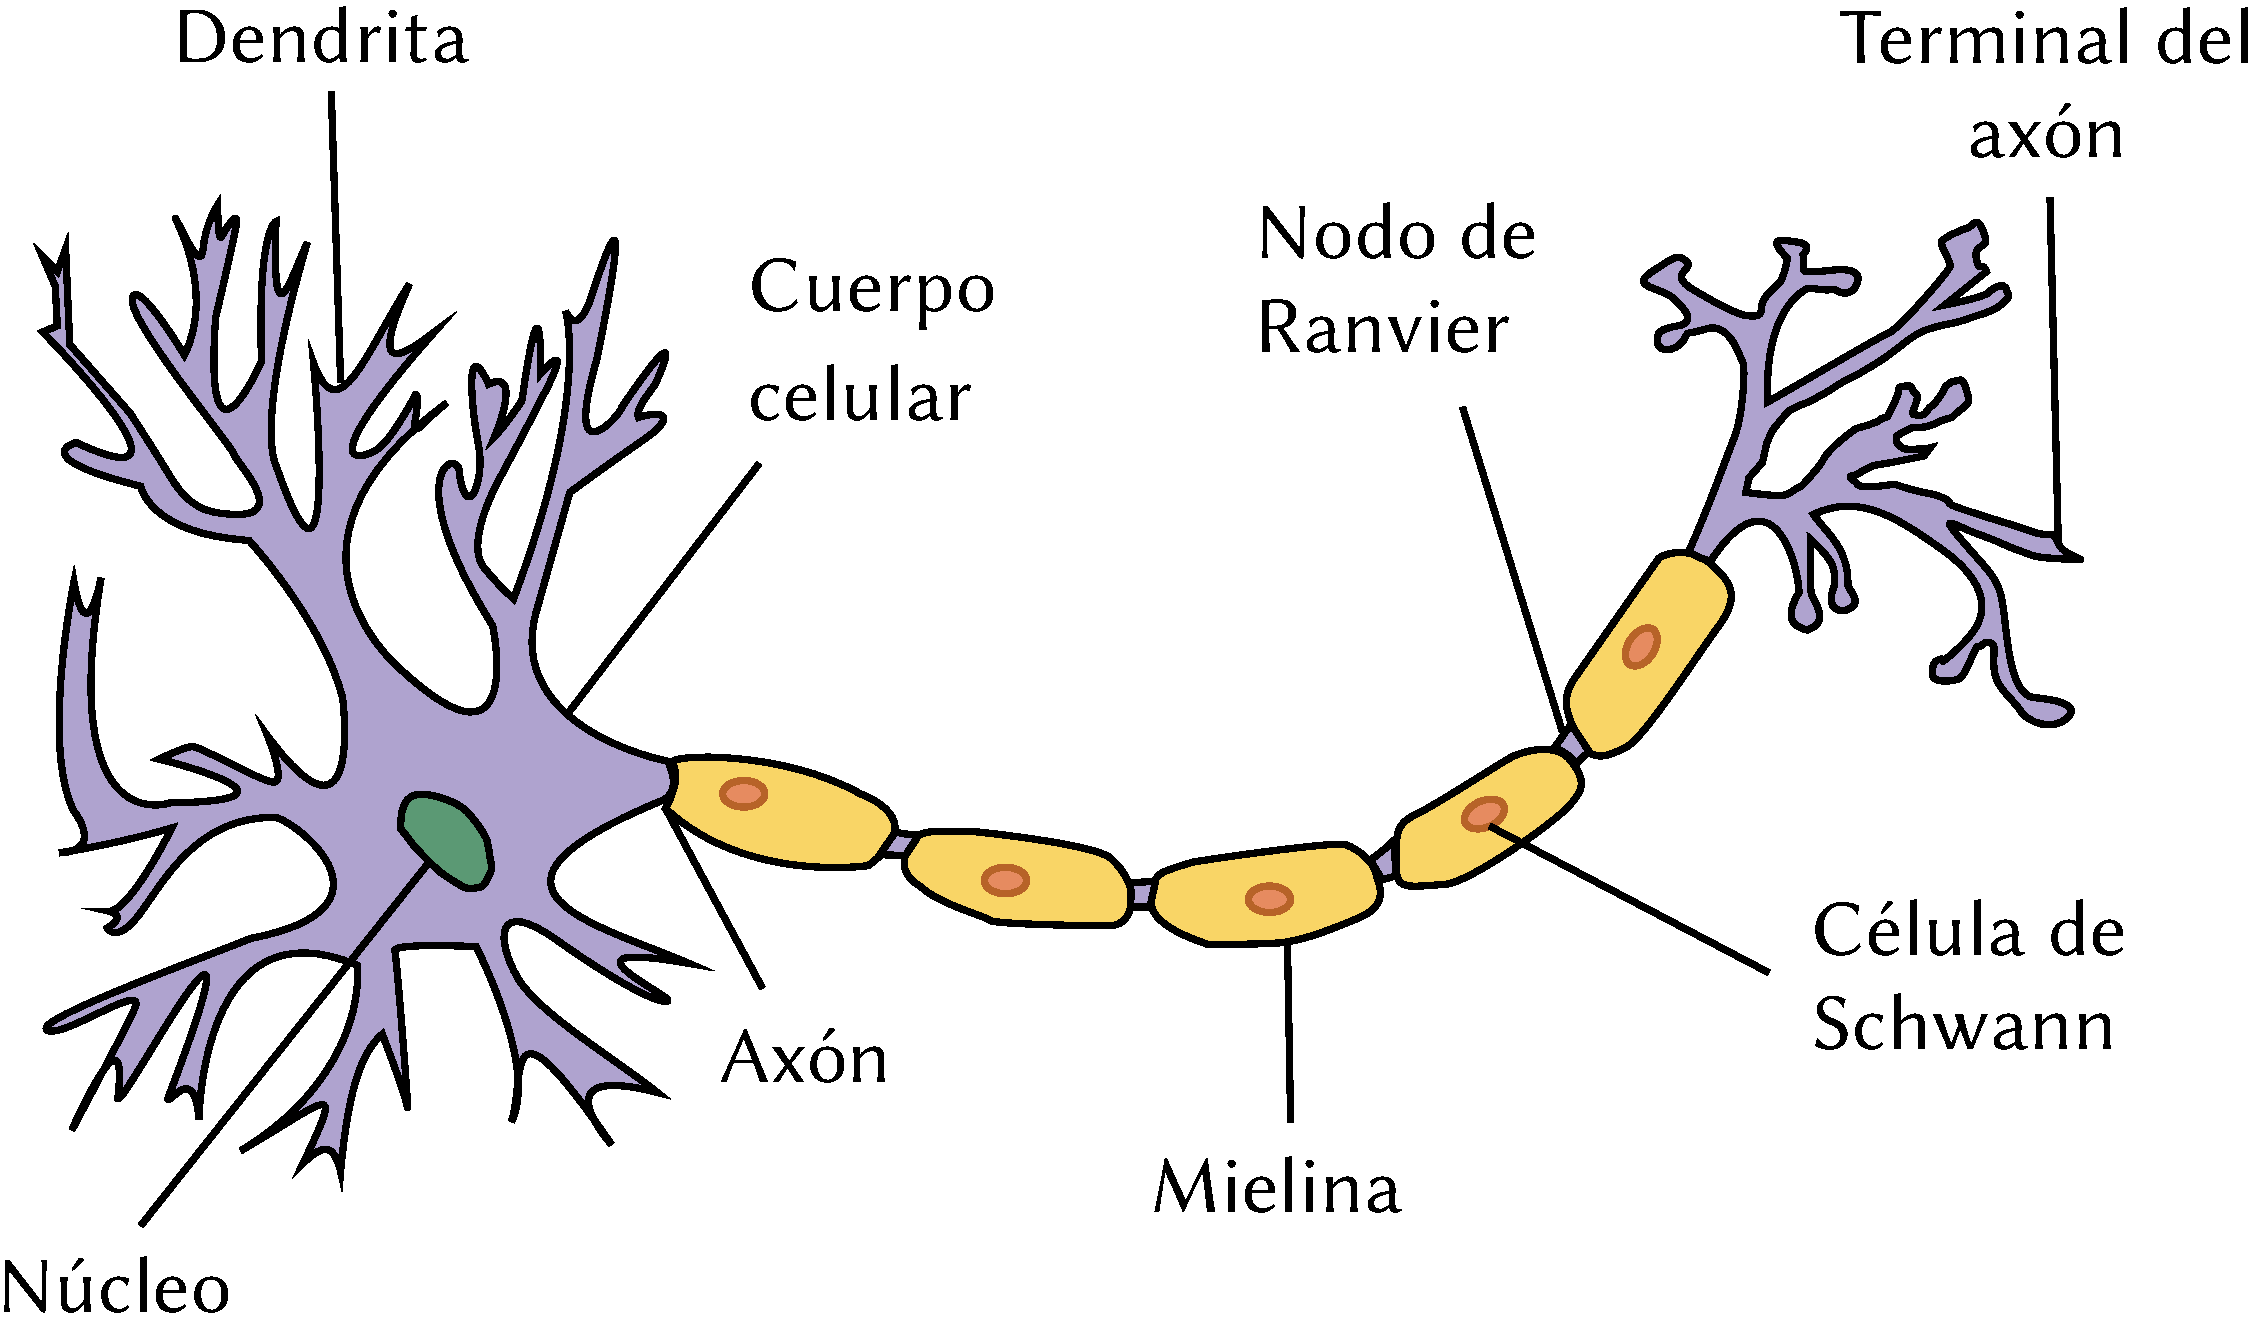
\includegraphics[width=0.7\textwidth]{img/neurona}
    \caption{Estructura de una neurona. Basada en \parencite{dhp1080_neurona_2007}.}
    \label{fig:neurona}
  \end{figure}
\end{frame}

\begin{frame}{Redes neuronales biológicas}
  \begin{itemize}
    \item Las neuronas se envían señales entre sí mediante un proceso electroquímico denominado sinapsis.
    \item La neurona presináptica (emisora) libera los neurotransmisores a través del axón y la neurona postsináptica (receptora) los capta a través de las dendritas.
    \item La tasa de envío por parte de la neurona presináptica depende de la proporción de dos tipos de sinapsis que esta reciba: \begin{itemize}
      \item sinapsis inhibidoras,
      \item sinapsis excitadoras.
    \end{itemize}
  \end{itemize}
\end{frame}

\section{Estructura y funcionamiento de las redes neuronales}

\begin{frame}{Neurona de McCulloch-Pitts}
  \begin{itemize}
    \item Modelo computacional. Múltiples entradas a una unidad de procesamiento y una sola salida.
    \item Cada entrada puede tomar el valor 0 o 1 y puede ser de tipo excitador o inhibidor. \begin{itemize}
      \item Si alguna de ellas es inhibidora y transmite el valor 1, la salida es 0.
      \item Si no hay conexiones inhibidoras activadas, se suman las entradas. Si dicha suma es mayor que el valor umbral, la salida es 1, en otro caso, 0.
    \end{itemize}
  \end{itemize}
\end{frame}

\begin{frame}{Neurona de McCulloch-Pitts}
  \begin{figure}[h]
    \centering
    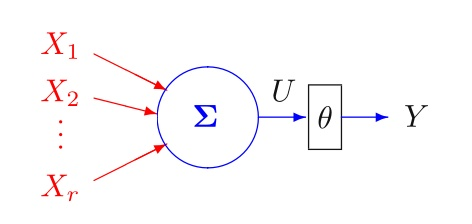
\includegraphics[width=.7\textwidth]{img/mcculloch-pitts}
    \caption{Neurona de McCulloch-Pitts con $r$ entradas binarias $X_1,\dots,X_r$, una salida binaria $Y$ y un umbral $\theta$. Extraída de \parencite{izenman_modern_2008}.}
    \label{fig:mcculloch-pitts}
  \end{figure}
\end{frame}

\begin{frame}{Neurona de McCulloch-Pitts}
  \begin{itemize}
    \item Divide el espacio de entrada en dos mitades según el hiperplano $\sum_j X_j = \theta$.
    \item Se puede representar cualquier función booleana mediante combinaciones de neuronas.

    \vspace{1em}

    \begin{figure}[h]
    \centering
    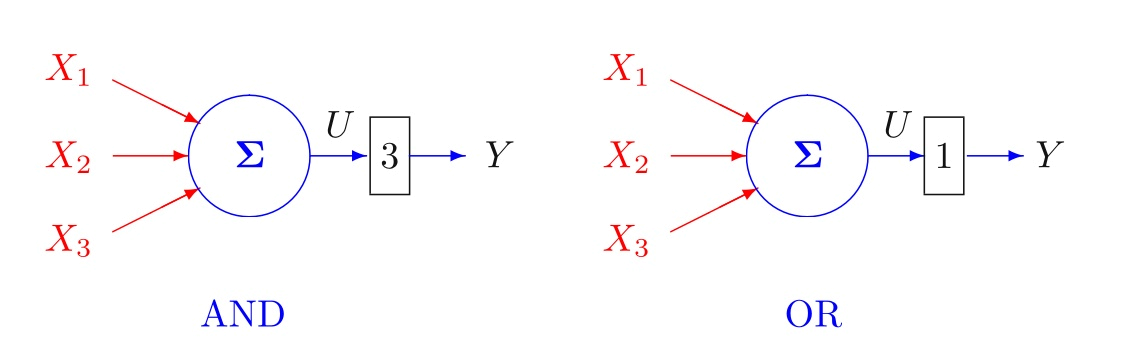
\includegraphics[width=.8\textwidth]{img/and-or}
    \caption{Neuronas de McCulloch-Pitts representando las funciones lógicas AND y OR. Extraída de \parencite{izenman_modern_2008}.}
    \label{fig:and-or}
  \end{figure}
  \end{itemize}
\end{frame}

\begin{frame}{Neurona de McCulloch-Pitts}
  \begin{itemize}
    \item Este modelo no es adecuado para realizar un proceso de aprendizaje ya que hay que cambiar los valores de la neurona para resolver diferentes problemas.
    \item Se perdió pronto el interés en este modelo computacional y se desarrollaron otros.
  \end{itemize}
\end{frame}

\begin{frame}{Perceptrón de una capa}
  \begin{itemize}
    \item Neurona de \textit{McCulloch-Pitts} con pesos $\beta_i \in \mathbb{R}$ por cada conexión.
    \item Si $\beta_i > 0$ la conexión es excitadora.
    \item Si $\beta_i < 0$ la conexión es inhibidora.
    \item Si  $\beta_i = 0$ no hay conexión.
    \item Suma ponderada $U = \sum_j \beta_j X_j$ que se compara con el umbral. Se puede eliminar este último añadiendo un sesgo $\beta_0 = - \theta$ y una variable $X_0 = 1$.
  \end{itemize}
\end{frame}

\begin{frame}{Perceptrón de una capa}
  \begin{figure}[h]
    \centering
    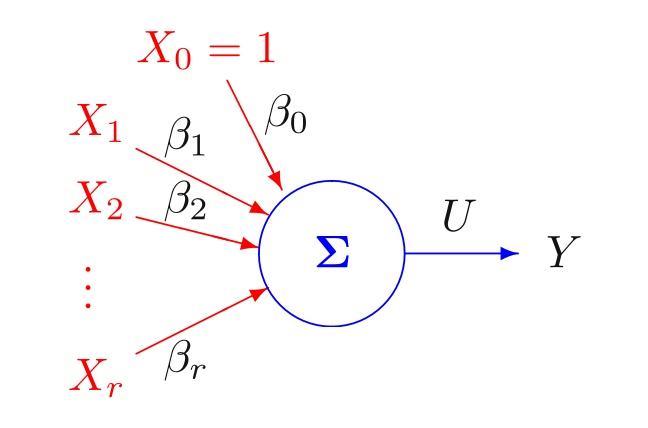
\includegraphics[width=.7\textwidth]{img/perceptron}
    \caption{Perceptrón de $r$ entradas binarias con pesos $\{\beta_j\}$ y salida binaria $Y$. Incluye el término de sesgo $\beta_0$. Extraída de \parencite{izenman_modern_2008}.}
    \label{fig:perceptron}
  \end{figure}
\end{frame}

\begin{frame}{Perceptrón de una capa}
  \begin{itemize}
    \item Si los datos de entrada son linealmente separables, se puede interpretar como un algoritmo de clasificación binaria: divide los datos según el hiperplano $U=0$.
    \item Si no son linealmente separables, la función asociada no es computable por un perceptrón.
  \end{itemize}
  \vspace{1em}

\begin{figure}[h]
  \centering
  \begin{subfigure}[b]{0.4\textwidth}
    \centering
    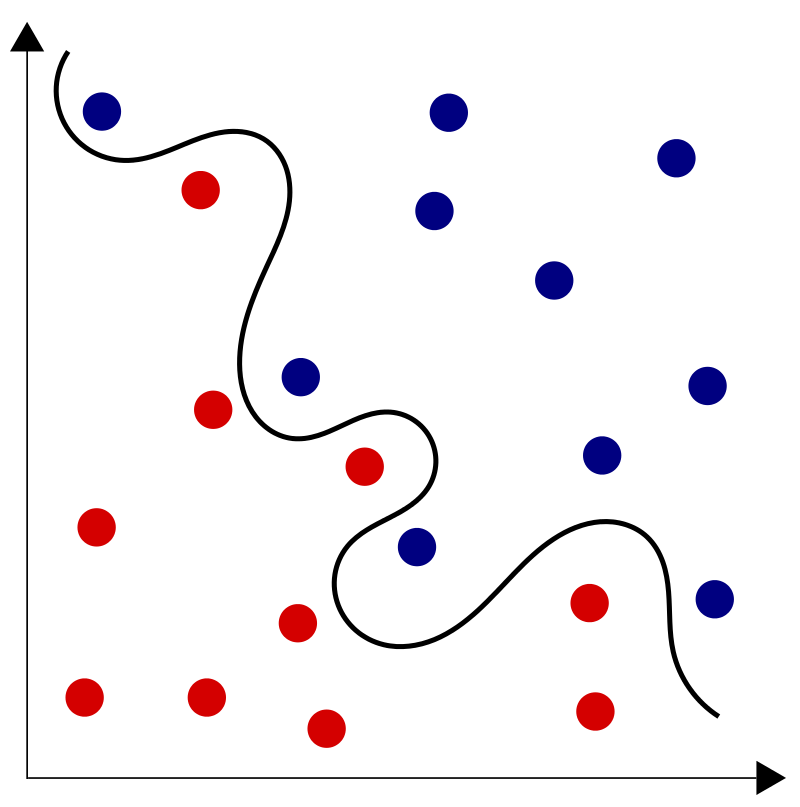
\includegraphics[width=.6\textwidth]{img/non-separable}
    \caption{No linealmente separables}
  \end{subfigure}
  \qquad
  \begin{subfigure}[b]{0.4\textwidth}
    \centering
    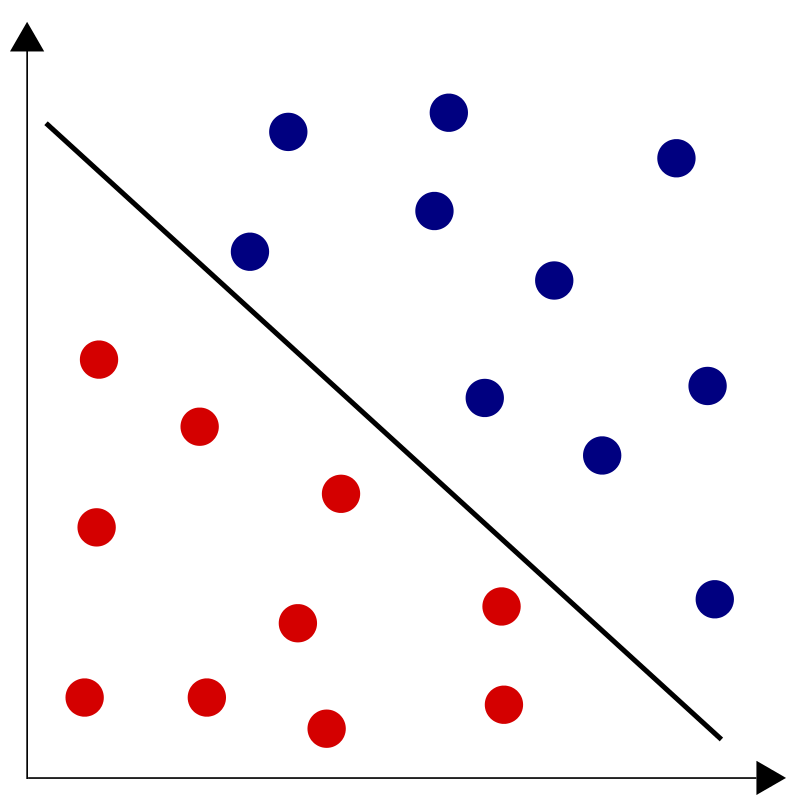
\includegraphics[width=.6\textwidth]{img/separable}
    \caption{Linealmente separables}
  \end{subfigure}
  \caption{Ejemplos de datos bidimensionales separables y no separables linealmente. Extraída de \parencite{wikipedia_separable}.}
  \label{fig:separable}
\end{figure}
\end{frame}

\begin{frame}{Redes de una capa}
\begin{itemize}
  \item Podemos considerar una red de perceptrones interconectados organizados en dos grupos: nodos de entrada $\{X_j\}$ y nodos de salida $\{Y_k\}$, con valores reales o discretos.
  \item Cada conexión $X_j \to Y_k$ tiene un peso $\beta_{jk}$.
  \vspace{1em}

    \begin{figure}[h]
    \centering
    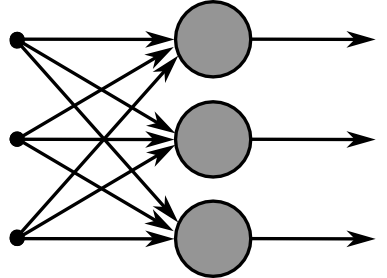
\includegraphics[width=.5\textwidth]{img/single}
    \caption{Esquema de red con perceptrones de una capa. Extraída de \parencite{wiki_single_2015}.}
    \label{fig:perceptron}
  \end{figure}
\end{itemize}
\end{frame}

\begin{frame}{Funciones de activación}
  \begin{itemize}
    \item Si tenemos datos de entrada $X=(X_1, \cdots , X_r)^T$ y $s$ nodos de salida, para cada uno de ellos hemos hecho
    $$U_k = \beta_{0k} + X^T \beta_{k} , \quad k = 1, \dots , s $$
    \item Necesidad de introducir no linealidad. Consideramos una función $f$ no lineal para la salida:
    $$ U_k = f(\beta_{0k} + X^T \beta_k) \quad k = 1, \dots , s$$
  \item Funciones de activación usuales: sigmoides como la logística o la tangente hiperbólica.
  \item Para clasificación binaria podemos usar la función signo. Para clasificación multiclase se introduce una función vectorial \textit{softmax}:

  $$f(x)_i = e^{x_i}/\sum_{k=1}^s e^{x_k}$$
\end{itemize}
\end{frame}

\begin{frame}{Funciones de activación: ReLU}
  \begin{itemize}
    \item Actualmente se usa la función $f(x) = \max \{0, x\}$, conocida como \textit{Rectified Linear Unit}.
  \end{itemize}

    \begin{figure}[h]
    \centering
    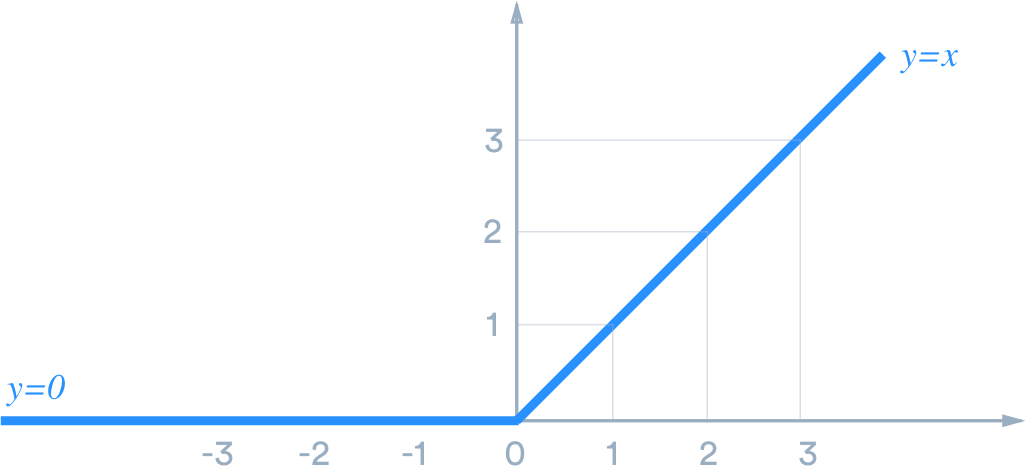
\includegraphics[width=.75\textwidth]{img/relu}
    \caption{Gráfica de la función ReLU.}
  \end{figure}

\end{frame}

\begin{frame}{Proceso de aprendizaje}
\begin{itemize}
\item Suponemos una serie de ejemplos de dos clases $\Pi_1$ y $\Pi_2$. Diremos que $X \in \Pi_1$ si y solo si $X^T\beta \ge 0$.
\item Utilizamos el conocimiento de la clase correcta para ir pasando ejemplos por la red y predecir la clase a la que pertenece cada uno.
\item Corregimos los pesos en cada iteración si se detecta un error.
\item Una solución será un vector de pesos $\beta^\ast$ que clasifique correctamente todos los ejemplos.
\end{itemize}
\end{frame}

\begin{frame}{Proceso de aprendizaje}
\begin{itemize}
\item Para una sucesión de entradas $\{X_h\}$, regla para actualizar los pesos en cada iteración es la siguiente:
  \begin{enumerate}
    \item Si la versión actual de los pesos $\beta_h$ consigue clasificar correctamente $X_h$, no cambiamos los pesos para la siguiente iteración.
    \item Si con los pesos $\beta_h$ no obtenemos una clasificación correcta, hacemos:
    $$\beta_{h+1} = \beta_h + \eta \, \operatorname{signo}(X^{t}_{h} \beta_h)X_h $$
  \end{enumerate}
  \item El parámetros $\eta > 0$ se conoce como \textit{learning rate}.
\end{itemize}
\end{frame}

\begin{frame}{Proceso de aprendizaje}
  \begin{itemize}
    \item \textbf{Teorema (Convergencia del perceptrón). } Para un problema de clasificación binaria con clases linealmente separables, si existe una solución $\beta^\ast$, el algoritmo descrito anteriormente la encontrará en un número finito de iteraciones.
  \end{itemize}
\end{frame}

\begin{frame}{Perceptrón multicapa}
  \begin{itemize}
    \item Se distribuyen los nodos en varias capas y se aplican transformaciones no lineales en el paso de una capa a la siguiente.
    \item Dos tipos:
    \begin{itemize}
      \item Capas totalmente contectadas.
      \item Capar parcialmente conectadas.
    \end{itemize}
  \end{itemize}
  \begin{figure}[h]
    \centering
    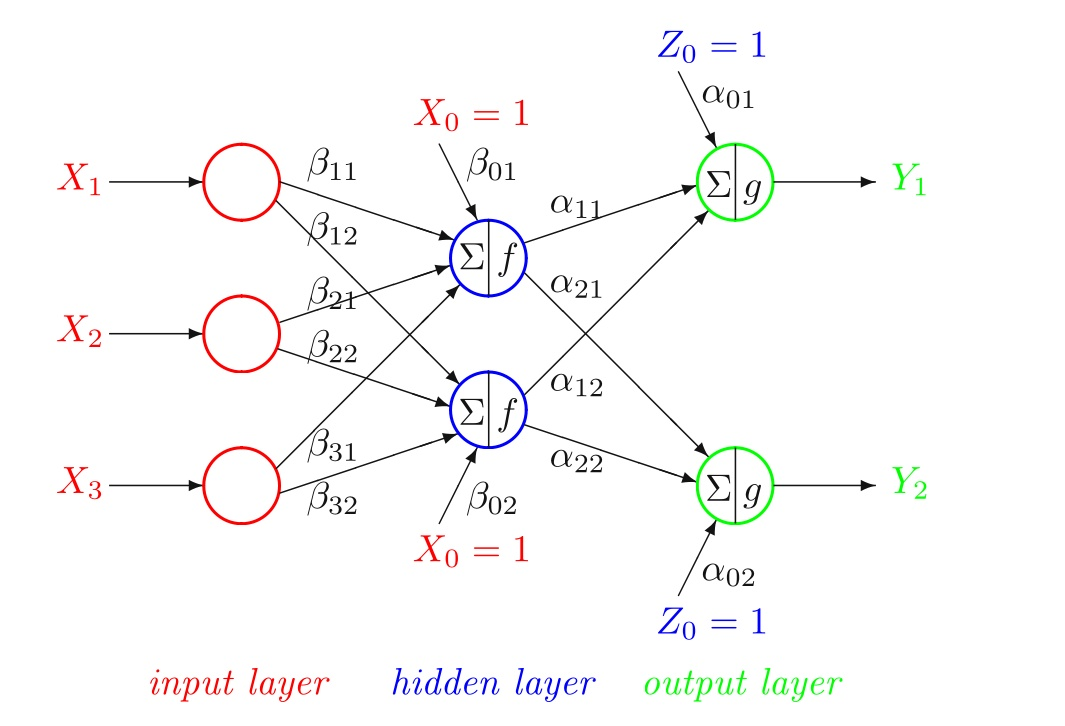
\includegraphics[width=.7\textwidth]{img/multicapa}
  \end{figure}
\end{frame}

\begin{frame}{Perceptrón multicapa}
  \begin{itemize}
    \item Para el proceso de aprendizaje de la red, se utiliza la técnica de gradiente descendente.
    \item Una vez conseguida pesos \textit{suficientemente buenos} se puede utilizar la red para clasificar nuevos ejemplos.
    \item También se puede abordar el problema de regresión lineal.
    \item Desventaja: pérdida de interpretabilidad frente a modelos clásicos.
    \item Ventaja: consiguen resolver problemas mucho más complejos.
  \end{itemize}
\end{frame}

\begin{frame}{Principales problemas}
\textbf{Overfitting}: La red ha memorizado los ejemplos de capacitación, pero no ha aprendido a generalizar a nuevas situaciones.
  \begin{figure}[h]
    \centering
    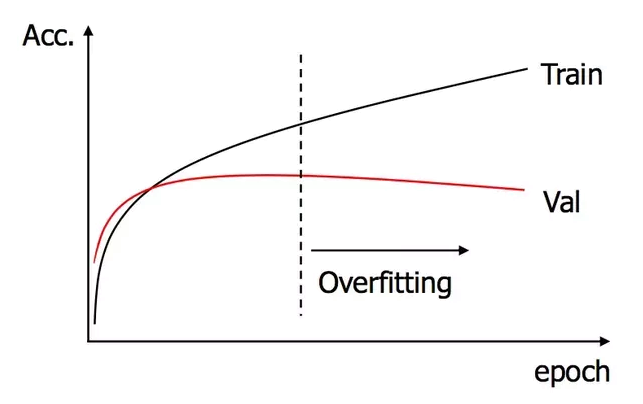
\includegraphics[width=.6\textwidth]{img/overfitting}
  \end{figure}
\end{frame}
\begin{frame}{Principales problemas}
\textbf{Learning rate}: Indica cuanto hay que cambiar el modelo en respuesta al error estimado cada vez que actualizan los pesos de este.
  \begin{figure}[h]
    \centering
    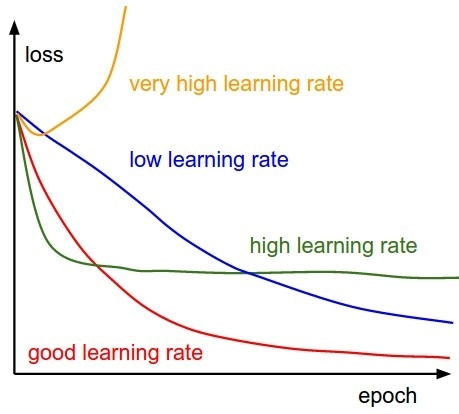
\includegraphics[width=.6\textwidth]{img/learning-rate}
  \end{figure}
\end{frame}

\begin{frame}{Teorema de aproximación universal}
El teorema de aproximación universal establece que una red feed-forward con una sola capa oculta que contiene un número finito de neuronas puede aproximarse a funciones continuas en subconjuntos compactos de $R_n$, bajo condiciones poco restrictivas sobre la función de activación.
Dos tipos:
\begin{itemize}
  \item Ancho acotado.
  \item Ancho no acotado.
\end{itemize}
\end{frame}

\begin{frame}{Clasificación de redes neuronales}
  \begin{itemize}
    \item Según el modelo de aprendizaje
      \begin{itemize}
      \item \textbf{Aprendizaje supervisado}. El conjunto de entrenamiento se
        encuentra <<etiquetado>>.
      \item \textbf{Aprendizaje no supervisado}. Minimizar una función de coste.
      \item \textbf{Aprendizaje por refuerzo}. La red busca maximizar una función de
        recompensa <<acumulada>>.
      \end{itemize}
    \item Según su topología\\
      Presenta ciclos, totalmente conectada, neuronas conectadas consigo mismas...
  \end{itemize}
\end{frame}

\begin{frame}{Autoencoders}
\begin{itemize}
\item Aprendizaje no supervisado.
\item Codifica la entrada.
\item Busca copiar su entrada en la salida. Está formado por:
  \begin{itemize}
    \item Codificador
    \item Decodificador
  \end{itemize}
\end{itemize}
\begin{figure}[h]
  \centering
  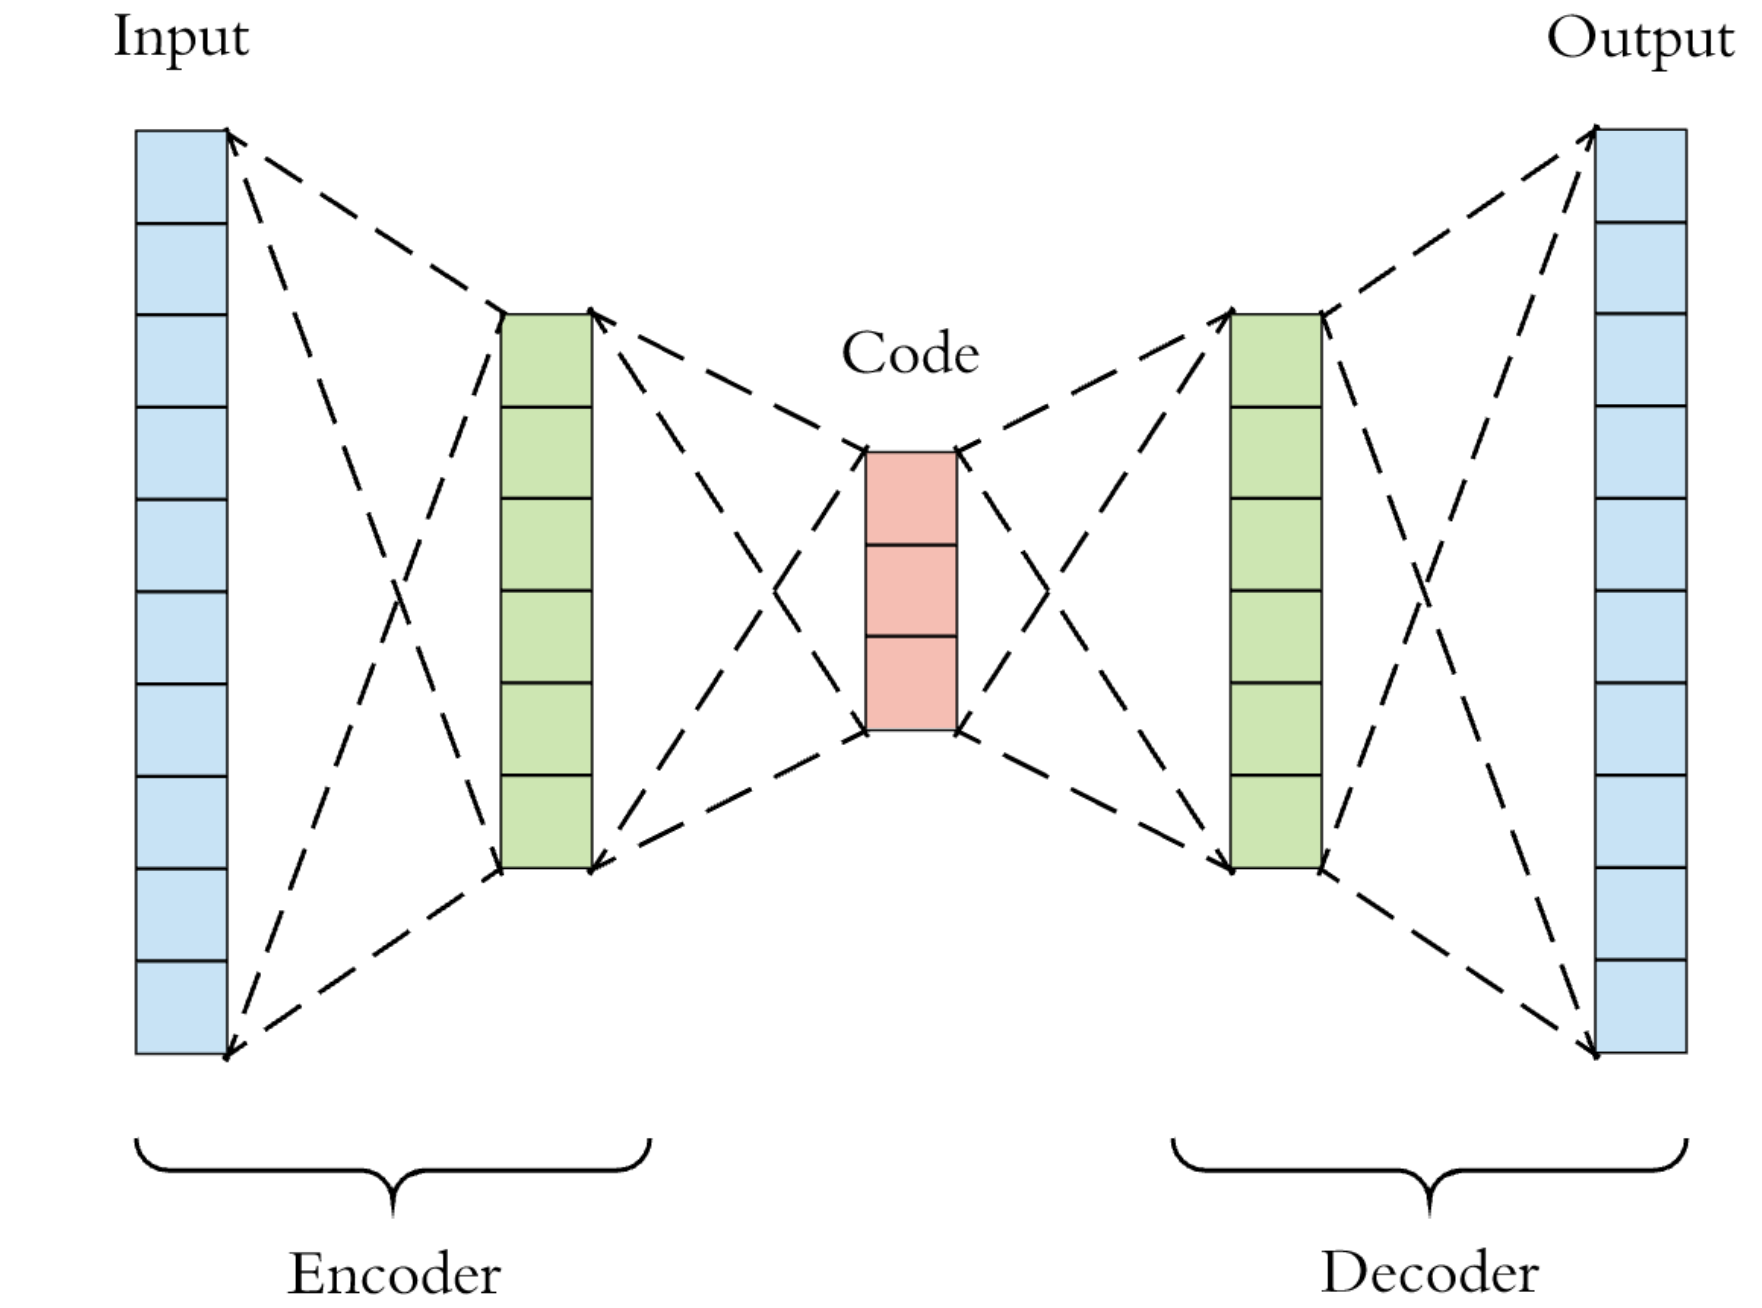
\includegraphics[width=.6\textwidth]{img/autoencoder}
\end{figure}
\end{frame}

\begin{frame}{Ejemplo reducción de dimensión}
    Base de datos MNIST, números escritos a mano.\\
  Imagenes originales $28\times28 \implies \mathbb{R}^{784}$.
\begin{figure}[h]
  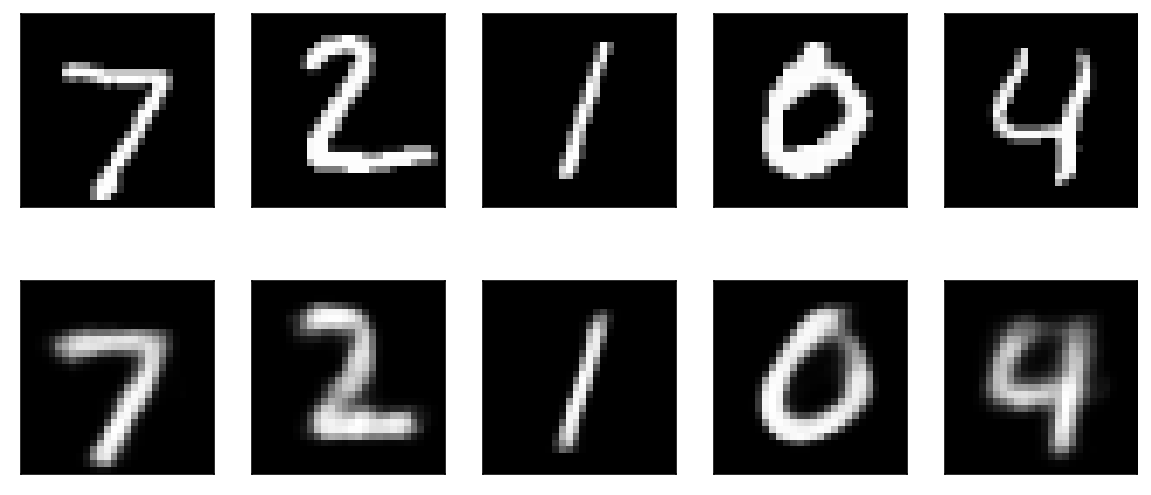
\includegraphics[width=.6\textwidth]{img/autoencoder_ex1}
\end{figure}
Imagenes reconstruidas.\\

Codificación en $\mathbb{R}^4$. Primera imagen: $\{13.325841, 16.394411, 13.2127905, 0.90243316\}$
\end{frame}

\begin{frame}{Ejemplo eliminación de ruido}
Entrenamos la red con imágenes con ruido como entrada e imágenes sin ruido como
salida deseada.
\begin{figure}[h]
  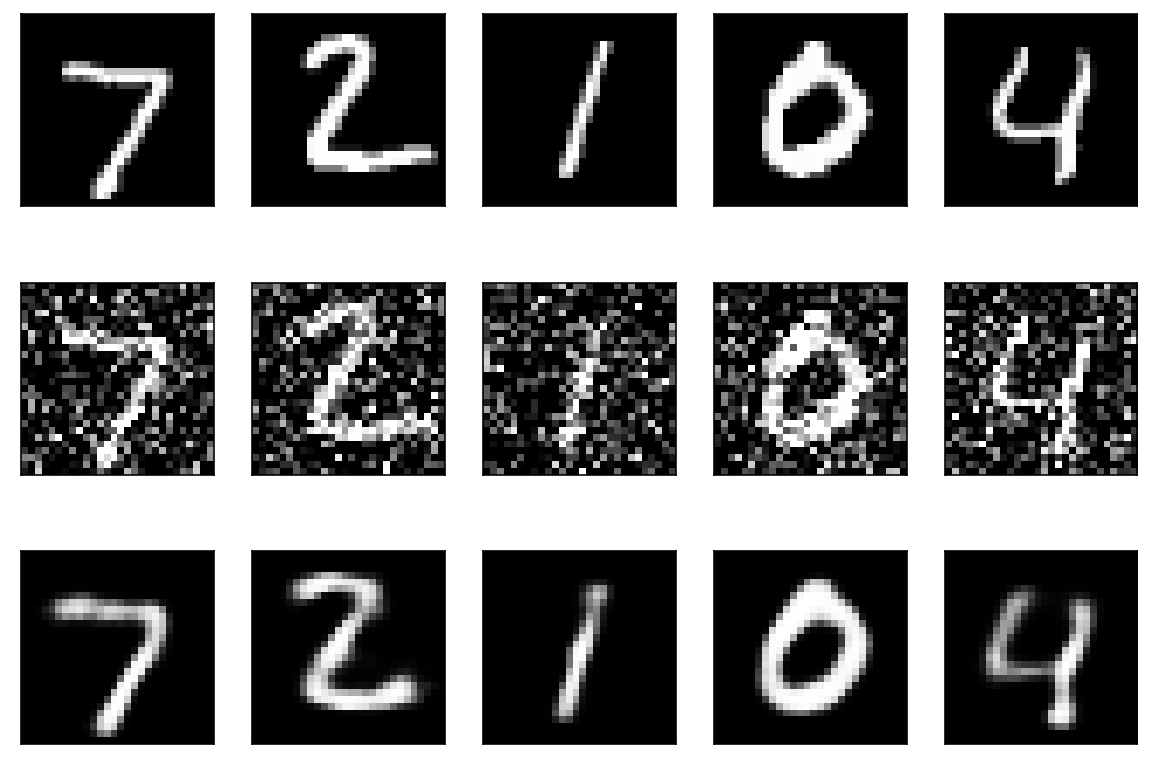
\includegraphics[width=.6\textwidth]{img/autoencoder_ex2}
\end{figure}
\end{frame}

\begin{frame}{Redes convolucionales}
    \begin{itemize}
        \item Uno de los problemas principales de las redes neuronales convencionales en el tratamiento de imágenes es el gran número de parámetros.
        \item La solución más extendida son las redes convolucionales.
    \end{itemize}
\end{frame}

\begin{frame}{Redes convolucionales}
  \begin{itemize}
    \item Convolución: consiste en «desplazarse» por todas las posibles posiciones de una matriz, y aplicar el producto elemento a elemento entre la submatriz y el filtro seleccionado.

    \begin{figure}[h]
      \centering
      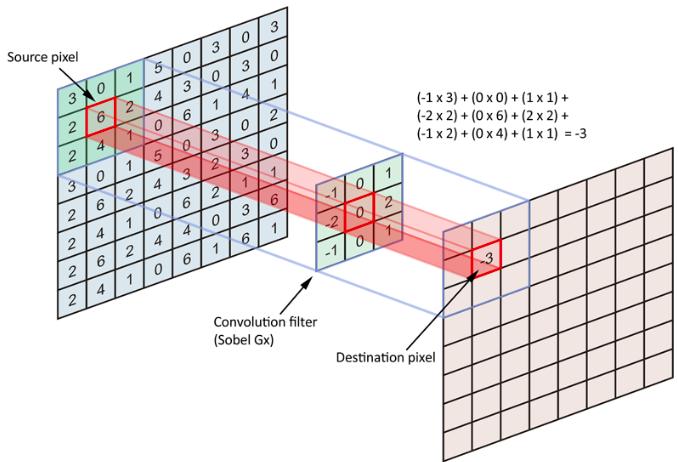
\includegraphics[width=.6\textwidth]{img/conv}
    \end{figure}
  \end{itemize}
\end{frame}

\begin{frame}{Redes convolucionales}
    \begin{itemize}
        \item Las capas más externas extraen características más generales.
        \item Las capas más profundas extraen características más específicas.
        \item Al final se añade una capa completamente conectada que realiza la clasificación de las imágenes.
    \end{itemize}
\end{frame}

\begin{frame}{Redes Neuronales Recurrentes}
\begin{itemize}
\item Son una de las variantes de redes más importantes utilizadas en procesamiento
de lenguaje natural.
\begin{figure}[h]
  \centering
  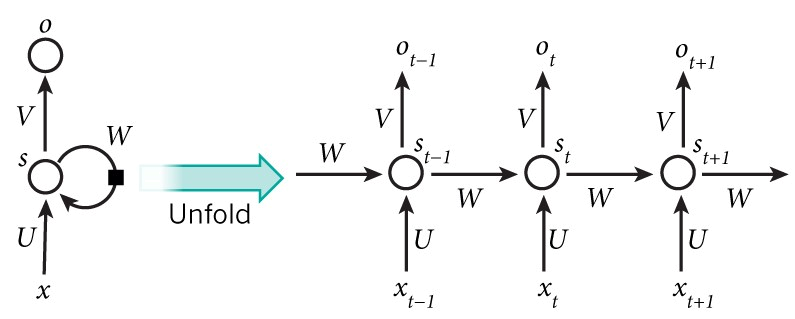
\includegraphics[width=.6\textwidth]{img/rnn}
\end{figure}
\end{itemize}
\end{frame}

\begin{frame}{CIFAR-10}
\begin{itemize}
  \item El conjunto de datos CIFAR-10 tiene 60000 imágenes en color de 32x32 píxeles divididas en 10 clases, con 6000 imágenes por clase. El conjunto se divide en 50000 imágenes para el conjunto de entrenamiento y 10000 imágenes en el conjunto de test.
  \begin{figure}[h]
    \centering
    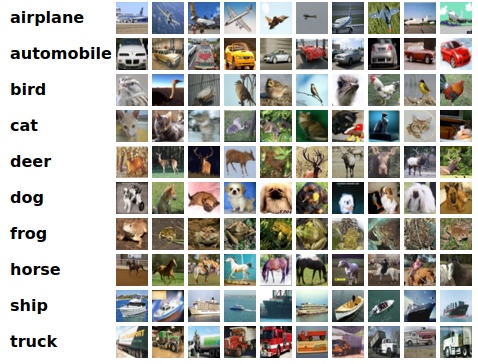
\includegraphics[width=.6\textwidth]{img/cifar10}
  \end{figure}
\end{itemize}

\end{frame}

\begin{frame}[t,allowframebreaks]{Referencias}
  \printbibliography[heading=none]
\end{frame}

\end{document}
